\documentclass{article}
\usepackage[margin=1in]{geometry} % Définit la marge à 1.5 pouces
\usepackage{amsmath}
\usepackage{graphicx}

\title{Revu littéraire}
\author{Auteur : SABIDANI YENTEM ELISEE}

\begin{document}

	\maketitle
	
	\newpage
	\tableofcontents
	\newpage

	\section{Thème 1 : Vers un modèle sémantique pour la gestion de l´interopérabilité dans le domaine de l´agriculture.(Auteur : MOUALKIA AMMAR)}
	
	\section{Chapitre 01 : État de l'art et travaux connexes}
	
	\subsection{Introduction}
	Dans la première partie de ce chapitre, nous commencerons par la description du
	problème majeur entre les systèmes de gestion dans le domaine de l’agriculture, en présentons
	quelques définitions de l’interopérabilité, ainsi son importance pour assurer une meilleure
	efficacité opérationnelle pour ces systèmes. Ensuite on va examiner l'état de l'art des concepts
	de base, en définissant le concept d'ontologie et en soulignant son efficacité en termes de
	représentation sémantique et formelle des données. Par la suite, nous présenterons une
	description et une évaluation des méthodologies de développement des ontologies, ce qui nous
	permettra d'identifier les faiblesses de ces méthodologies par rapport aux autres approches.
	
	\subsection{L’interopérabilité}
	L'interopérabilité est un défi majeur dans le domaine de la gestion de l'information et
	des systèmes informatiques. Elle fait référence à la capacité des différents systèmes à échanger
	des données et à collaborer de manière transparente et efficace.
	
	Il convient généralement d’identifier trois (03) types d’interopérabilité :
	\begin{itemize}
		\item L’interopérabilité technique : Elle concerne les problèmes techniques de liaison entre systèmes, la
		définition des interfaces, le format des données et les protocoles, y compris les
		télécommunications. Elle décrit la capacité pour des technologies différentes à
		communiquer et à échanger des données basées sur des normes d'interface bien
		définies et largement adoptées.
		
		\item L’interopérabilité sémantique :
		Elle assure que la signification exacte des informations échangées soit
		compréhensible par n’importe quelle autre application, même si celle-ci n’a pas été
		conçue initialement dans ce but précis. En effet, des conflits sémantiques surviennent
		lorsque les systèmes n’utilisent pas la même interprétation de l’information qui est
		définie différemment d’une organisation à l’autre. Pour réaliser l'interopérabilité
		sémantique, les deux côtés doivent se référer à un modèle de référence d'échange
		d'informations commun
		
		\item L’interopérabilité syntaxique :
		La syntaxe traduit le sens en symboles. Il y a entre la sémantique et la syntaxe
		le même rapport qu'entre le fond et la forme. L’interopérabilité syntaxique concerne
		la façon dont sont codées et formatées les données en définissant notamment la
		nature, le type et le format des messages échangés, Elle conduit à la notion de
		système ouvert permettant d'assumer l'hétérogénéité des composants.
	\end{itemize}

	\subsection{Concepts de base}
	L'ontologie est une technique de modélisation des données pour un dépôt de données structuré,
	fondé sur une collection de concepts avec leurs relations sémantiques et leurs contraintes sur le
	domaine.
	
		L'objectif principal d'une ontologie est de capturer la signification et la sémantique des
	connaissances d'un domaine, afin de permettre une compréhension et une communication
	précises entre les humains et les machines basé sur des langages formels tels que RDF
	(Resource Description Framework) ou OWL (Web Ontology Language).
	
	\begin{itemize}
		\item OWL : Le langage OWL est une solution puissante et efficace pour la construction d'ontologies
		dans divers domaines. Son utilisation répandue témoigne de sa capacité à relever les défis liés
		à la représentation sémantique des connaissances et à l'interopérabilité des systèmes d'information.
		\item RDF : le RDF (Resource Description Framework) est un moyen de représenter des informations sur le web de manière structurée.
	\end{itemize}

	Les ontologies sont largement utilisées dans divers domaines tels que la santé, l'éducation,
	l'ingénierie, l'industrie, la finance, et bien d'autres encore.
	
	
	\subsection{Méthodologie de développement d´ontologies}
	Parmi ces approches, on peut citer la méthodologie de Gruninger et Fox
	, l'approche Methontology, l'approche de Noy et McGuinness, l'approche d'Uschold
	et King, ainsi que la méthodologie FAO-Based proposé dans le travail.
	
	\begin{itemize}
	\item Activités de pré-développement :
	
	\textbf{- Collecte et analyse d'informations de domaine :} Cette activité implique la recherche et la
	collecte d'informations pertinentes sur le domaine spécifique pour lequel l'ontologie est
	développée. Cela peut inclure l'examen de documents existants, l'interrogation d'experts du
	domaine, la consultation de bases de données et d'autres sources d'informations pertinentes.
	L'objectif est de rassembler les connaissances nécessaires pour construire une ontologie
	représentant le domaine de manière précise.
	
	\textbf{- Spécification des terminologies de l'ontologie : }Dans cette activité, les termes et les concepts
	clés du domaine sont identifiés et définis. Cela comprend la création d'une liste de termes, leur
	définition et leur organisation hiérarchique. La spécification des terminologies permet de créer
	une base solide pour la représentation des connaissances dans l'ontologie.
	
	\textbf{- Établissement de questions de compétence (en utilisant des logiques) : }Il s'agit de définir les
	questions de compétence qui seront utilisées pour vérifier la cohérence et l'expressivité de
	l'ontologie. Les questions de compétence sont formulées en utilisant des logiques formelles
	telles que la logique de description et la logique de premier ordre. Elles permettent de tester les
	règles et les inférences de l'ontologie afin de garantir sa qualité et son adéquation avec le
	domaine.
	
	\item Activités de développement :
	
	\textbf{- Formalisation d'ontologie :} Cette activité consiste à formaliser l'ontologie en utilisant un
	langage d'ontologie tel que RDF, OWL ou un autre langage approprié. La formalisation
	implique la création de classes, de propriétés, de relations et d'axiomes qui décrivent les
	concepts et les relations du domaine. Il peut également inclure l'utilisation de règles logiques
	pour exprimer des inférences et des contraintes dans l'ontologie.
	
	\textbf{- Évaluation d'ontologie :} L'évaluation de l'ontologie vise à vérifier sa qualité et son adéquation
	par rapport aux objectifs initiaux. Cela peut inclure des tests de cohérence logique, des
	évaluations de la couverture des concepts, des comparaisons avec d'autres ontologies similaires,
	et l'identification des lacunes ou des incohérences éventuelles. L'évaluation permet d'identifier
	les problèmes potentiels et d'améliorer l'ontologie en conséquence.
	
	\item Activités post-développement :
	
	\textbf{- Évolution d'ontologie :} L'évolution de l'ontologie fait référence aux modifications et aux
	mises à jour apportées à l'ontologie après son développement initial. Les ontologies peuvent
	nécessiter des ajustements au fil du temps en fonction de l'évolution du domaine, des nouvelles
	exigences ou des nouvelles connaissances acquises. Cette activité implique la gestion des
	versions, la gestion des changements et l'adaptation de l'ontologie pour qu'elle reste pertinente
	et utile dans le temps.
	\end{itemize}
	
	\subsection{Les Motivations de travail :}
	Pour la bonne marche du projet, plusieurs article on été exploité dans le cadre de la conception de notre ontologie.
	
	\subsection{Analyses et synthèse :}
	\subsubsection{Ontologies existantes pertinentes pour le domaine agricole}
	D'après notre analyse des travaux connexes présentés dans le tableau 1, la quasi-
	totalité des articles étudiés considère que l'utilisation de la modélisation ontologique représente
	la meilleure solution pour la représentation des données. Plusieurs solutions ont été proposées
	en utilisant des ontologies existantes, notamment :
	
	- L'ontologie AGROVOC est réutilisée dans les articles [2] , [10], [18], [20] et [27].
	
	- L'ontologie d'agriculture Agri-Ont est utilisée dans les articles [18],[31].
	
	- L'ontologie des tâches d'exploitation agricole AGROPTO est réutilisée dans l'article [5], où
	OntoUML est utilisé pour développer des modèles conceptuels afin de décrire les aspects d'une
	tâche complexe.
	
	- Dans les articles [26] et [28], l'ontologie des traits (TO) et l'ontologie de la Culture (CO) pour
	le blé sont utilisées. Les chercheurs ont également associé 246 traits de la base de données
	GrainGenes à 155 termes de la TO.
	
	- L'ontologie des maladies des plantes PDO, l'ontologie de la protection des plantes
	(PPOntology) et l'ontologie du riz (RO) sont utilisées dans l'article [11].
	
	- L'ontologie des réseaux de capteurs sémantiques SSN [37] est utilisée dans les articles [7],
	[18] et [21] pour le stockage des informations collectées par les capteurs. Par exemple, dans
	l'article [7], les capteurs d'humidité du sol sont utilisés pour enrichir le web sémantique dans le
	domaine de la gestion et de la lutte contre les ravageurs qui affectent le raisin.
	
	\subsubsection{Langages d’implémentation des ontologies}
	La majorité des articles [2], [3], [4], [5], [6], [7], [8], [9], [10],[11], [12], [18], [19], [20], [22], [23] ,
	[25], [27], [29], [30], [31] et [35] motivent l’utilisation du langage d'ontologie Web OWL pour la
	description des ontologies, ce langage représente les concepts des classes en générale, ainsi
	l’intégration des règles SWRL pour donner la forme sémantique aux systèmes.
	
	\subsection{Conclusion}
	Dans ce chapitre, nous avons examiné en détail l'état de l'art des ontologies dans le
	domaine de l'agriculture. Nous avons réalisé une analyse approfondie des travaux existants et
	des méthodologies utilisées pour le développement d'ontologies. Les ontologies ont prouvé leur
	capacité à améliorer les performances des systèmes de gestion agricole en permettant la mise
	en place de mécanismes de contrôle intelligents grâce à l'intégration de l'inférence.
	Cependant, nous avons identifié un manque de modèle sémantique spécifique pour la gestion
	des entrepôts de stockage dans le domaine agricole. Nous avons constaté un besoin d'un modèle
	qui réponde aux exigences nécessaires pour une gestion optimale des entrepôts. Dans le chapitre
	suivant, nous proposerons un modèle qui abordera spécifiquement cette problématique. Notre
	objectif sera de concevoir une ontologie qui permettra une gestion avancée et interopérable des
	entrepôts de stockage agricole, en prenant en compte les différentes dimensions et contraintes
	propres à ce domaine.
	
	\newpage
	
	\section{Chapitre 02 : Une Ontologie pour la gestion de l´interopérabilité dans
		les entrepôts de grains}
	
	\subsection{Introduction}
	Dans ce deuxième chapitre, nous aborderons en détail les étapes clés du développement
	de notre ontologie de domaine. Nous allons également concevoir un système qui exploite cette
	ontologie. Ce système utilisera les concepts, les relations et les entités définis dans l'ontologie
	pour faciliter la recherche, la gestion et l'analyse des connaissances dans le domaine spécifique
	de l'agriculture.
	
	\subsection{Développement de l´ontologie}
	\subsubsection{La collecte d´information}
	
		La collecte d'informations constitue la première étape du processus de développement
	de l'ontologie. Dans le cadre de notre travail, nous avons effectué une recherche approfondie et
	exploité un ensemble de sources d'informations pertinentes pour collecter les données
	nécessaires à la construction de notre ontologie. Ces sources comprenaient des articles
	scientifiques, des documents techniques, des rapports et des systèmes dans le domaine de
	l'agriculture et de la gestion des entrepôts de stockage des grains
	
	Tableau
	
	Une fois les informations collectées, nous avons utilisé un diagramme de classe pour
	structurer et organiser ces données de manière logique. Le diagramme de classe nous a permis
	de représenter les concepts clés, les relations et les attributs associés aux entités dans notre
	ontologie. Il nous a également aidés à définir les hiérarchies, les propriétés et les contraintes
	nécessaires pour modéliser efficacement les différents aspects de la gestion des entrepôts de
	stockage des grains (Figure suivante).
	
	\newpage
	
	\subsection{Diagramme de classe}
	\begin{figure}[h]
		\centering
		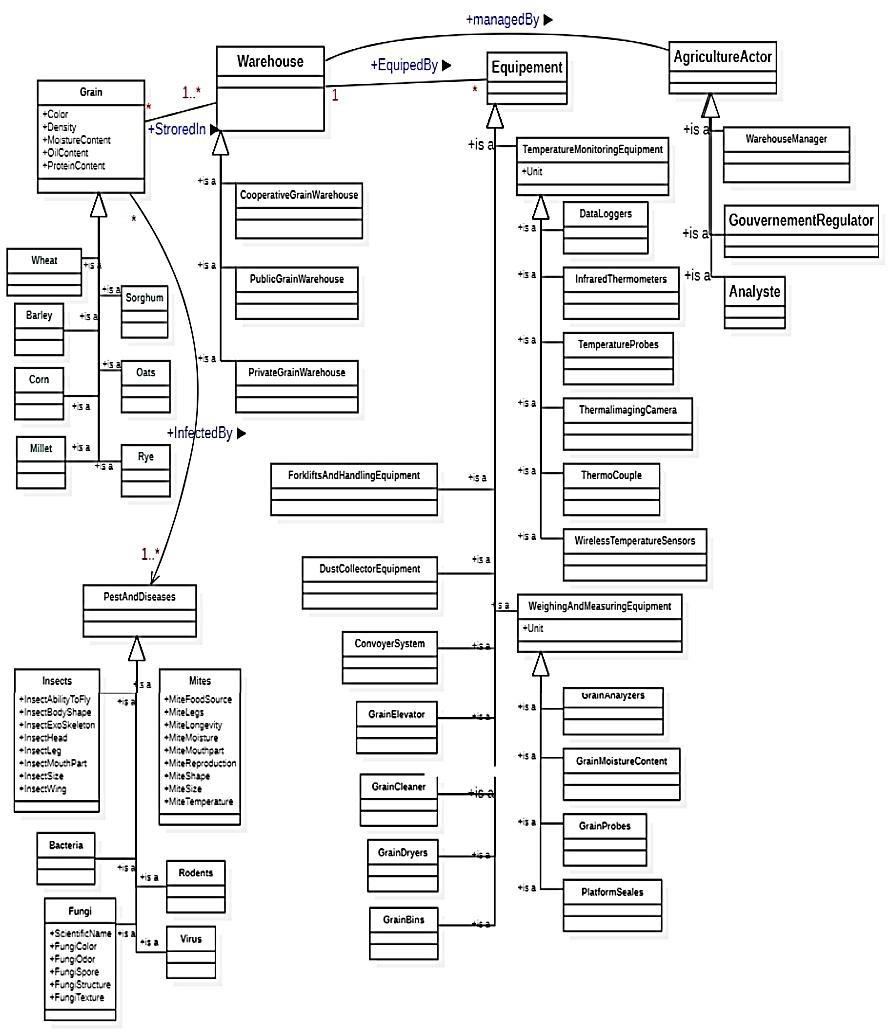
\includegraphics[width=0.7\textwidth]{uml.png}
		\caption{Diagramme de classe représentant la hiérarchie des concepts dans le domaine des entrepôts de grains}
		\label{fig:votre_image}
	\end{figure}
	
	L'utilisation d'un diagramme de classe nous a offert une représentation visuelle claire de
	la structure de notre ontologie, facilitant ainsi la compréhension et la communication des
	concepts et des relations entre les différents éléments. Il a également servi de guide lors des
	étapes ultérieures de développement, en fournissant une base solide pour la construction de
	l'ontologie et l'intégration des fonctionnalités requises.
	
	\subsection{La conceptualisation}
	Ici est listé et commenté tous les éléments du diagramme ULM précédent
	
	\subsection{Utilisation de l´ontologie proposée}
	\subsubsection{Acteurs et fonctionnalités offertes par le système :}
	\begin{itemize}
		\item Gestionnaires d'entrepôts de stockage des grains : Les gestionnaires d'entrepôts sont responsables de la gestion quotidienne des entrepôts de
		stockage des grains.
		\item Gouverneur : Ce gestionnaire est responsable de la supervision et de la gestion á grande échelle des
		entrepôts de stockage des grains.
		\item Analyste : Cet acteur est responsable de la gestion et le suivie des ravageurs et des maladies.
	\end{itemize}
	
	\subsection{Conclusion}
	Dans ce chapitre, nous avons réalisé une avancée significative en développant une
	ontologie spécifique pour le domaine du stockage de grains. Cette ontologie nous permet de
	représenter et de structurer les connaissances et les informations essentielles relatives à la
	gestion des entrepôts de stockage de grains de manière sémantique.
	
	\section{Chapitre 03 : Implémentation}
	
	\subsection{Introduction}
	Dans ce chapitre, nous décrivons les travaux applicatifs et les détails de mise en œuvre de
	notre travail. Nous allons décrire d'abord les outils et langage d'implémentation. Par la suite,
	nous détaillons les étapes de développement de notre système, et nous terminons par une
	présentation des fonctionnalités principales du système.
	
	\subsection{Mise en œuvre de la contribution}
	\subsubsection{Langages et outils de développement}
	Nous avons donc : Le langage Java Script, Le langage Python, Le navigateur Anaconda, Jupyter NoteBook, Visual Studio Code, Protégé(Pour l'ontologie)

	\subsubsection{Les bibliothèques utilisées}
	Owlready2(un package pour la programmation orientée ontologie en Python), Flask, React, Axios, Node.js, Material UI
	
	\subsection{Implémentation du système}
	Le développement de notre système se divise en trois parties principales : un backend,
	l’API et le front-end.
	Le backend concerne l’ontologie, l’API c’est l’intermédiaire et le front-end représente
	l’interface.
	
	\subsection{Implémentation de l’ontologie}
	\begin{figure}[h]
		\centering
		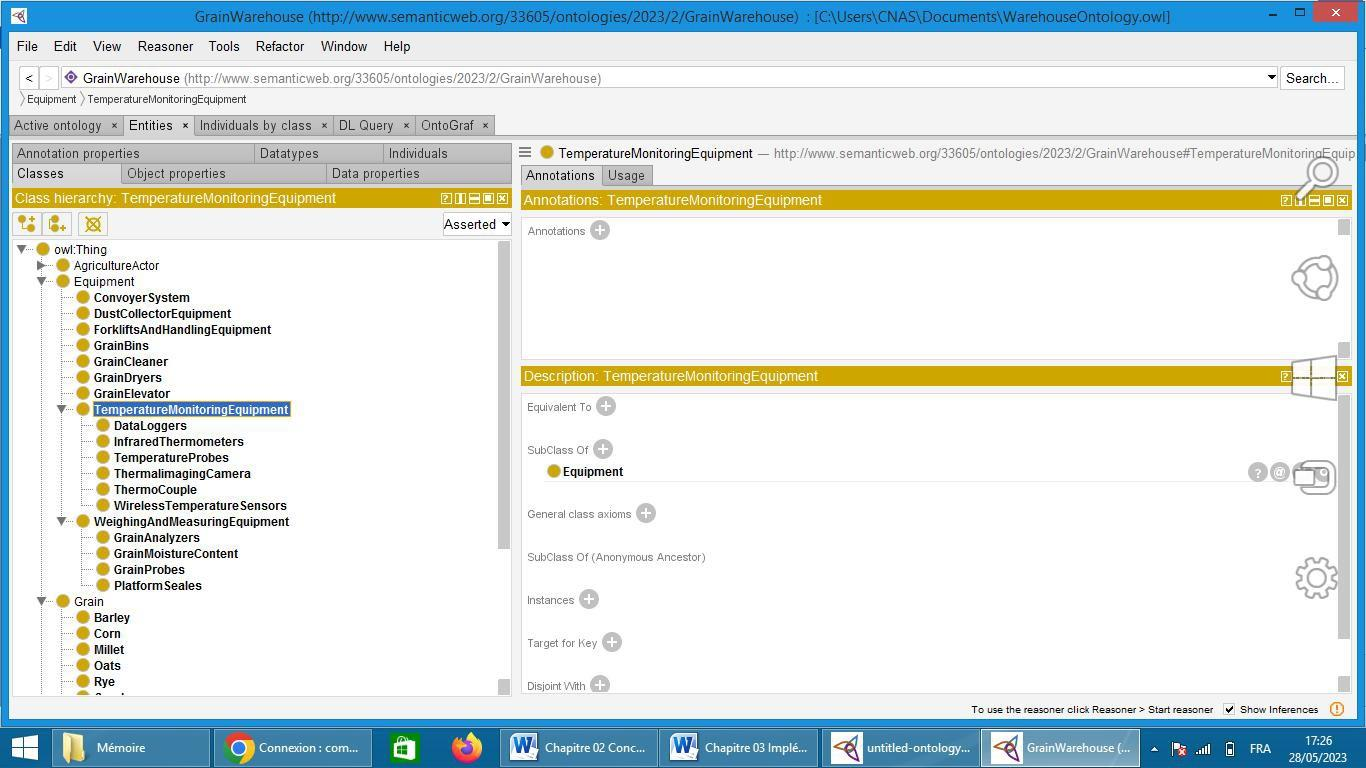
\includegraphics[width=0.7\textwidth]{onto1.png}
		\caption{Présentation des classes sous forme hiérarchique sur protégé}
		\label{fig:votre_image}
	\end{figure}

	\begin{figure}[h]
		\centering
		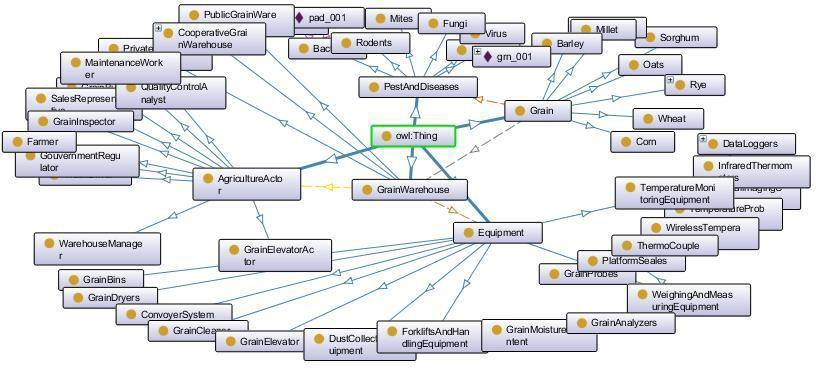
\includegraphics[width=0.7\textwidth]{onto2.png}
		\caption{Présentation des classes sous forme hiérarchique sur protégé}
		\label{fig:votre_image}
	\end{figure}

	\newpage

	\subsection{Implémentation de l’API}
	Une fois notre ontologie créée, nous passons à la création de l'API qui joue un rôle
	intermédiaire entre l'application Web et l'ontologie. L'API utilise différentes méthodes pour
	gérer l'ensemble des classes de l'ontologie. Dans le but d'exploiter au mieux le système, ces
	méthodes doivent inclure au moins les quatre opérations de base relatives à la gestion des
	données et des applications (CRUD) : Créer (Create), Lire (Read), Mettre à jour (Update) et
	Supprimer (Delete).
	Il as été implémenté avec python.
	
	\subsection{Implémentation de l’application Web}
	Après avoir créé et testé l'API, nous procédons à l'implémentation de l'application Web
	qui joue le rôle d'interface utilisateur. Nous avons utilisé React en tant que framework pour les
	fonctionnalités de manipulation, et Material-UI pour la création de l'ensemble des composants
	du site.
	
	\newpage
	
	\begin{figure}[h]
		\centering
		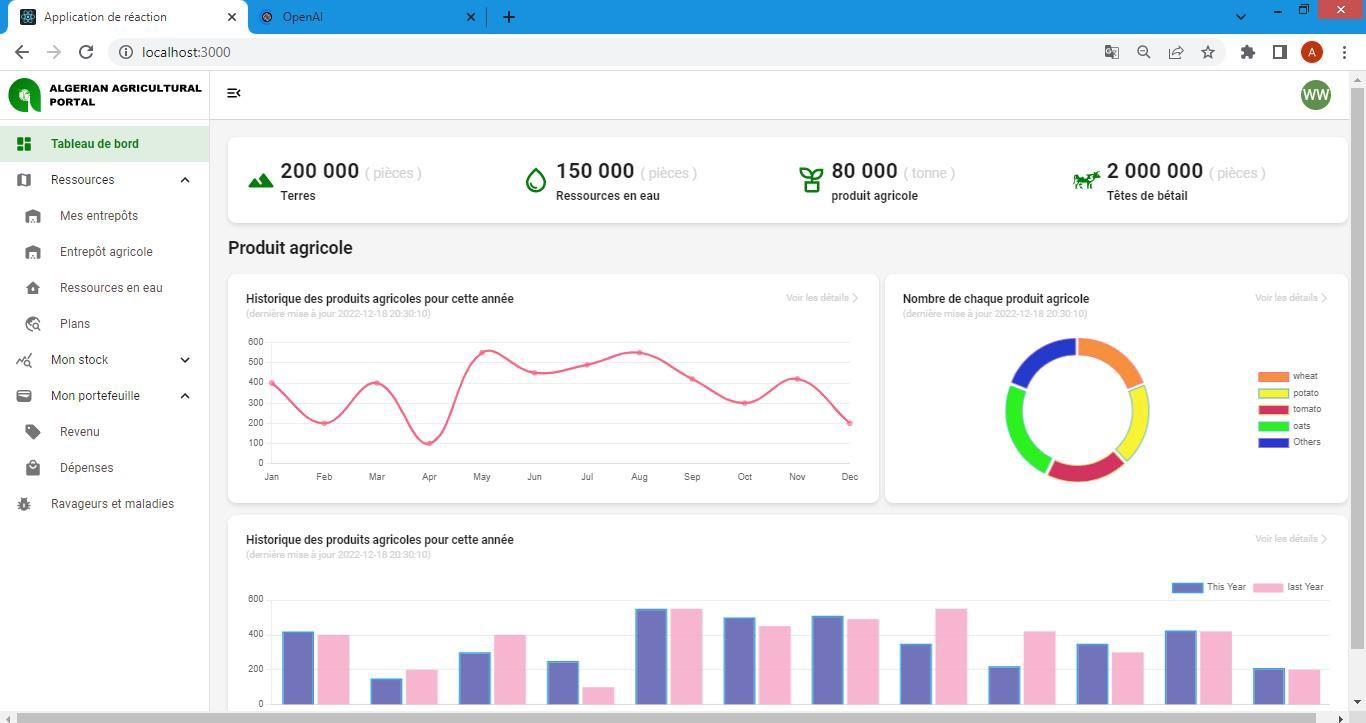
\includegraphics[width=0.7\textwidth]{tableau.png}
		\caption{Présentation des classes sous forme hiérarchique sur protégé}
		\label{fig:votre_image}
	\end{figure}

	\subsection{Conclusion}
	
		Dans ce chapitre, nous avons réussi à concrétiser notre conception en développant et en
	mettant en œuvre le système de gestion des entrepôts de stockage de grains basé sur l'ontologie
	que nous avons précédemment conçue. L'implémentation du système a été réalisée avec succès,
	en utilisant les technologies et les outils appropriés. Nous avons pu exploiter les fonctionnalités
	de l'ontologie pour organiser les données de manière sémantique et faciliter l'interprétation des
	informations liés au stockage des grains.
	
		Le système offre une interface conviviale permettant aux utilisateurs d'interagir
	facilement avec les fonctionnalités offertes. L'implémentation de ce système a apporté de
	nombreux avantages à la chaîne agricole et aux parties prenantes concernées.
	
	\subsection{Conclusion générale}
	Ce mémoire de fin d'études a apporté une contribution significative en abordant le
	problème de représentation sémantique des connaissances et la gestion d´interopérabilité. Grâce
	à une revue approfondie de la littérature et à l'utilisation de méthodologies bien établies, une
	ontologie dédiée aux entrepôts de stockage agricoles a été conçue, permettant une représentation
	précise des concepts, des relations et des propriétés spécifiques à ces infrastructures.
		
		L'application développée pour exploiter cette ontologie offre une interface intuitive et
	conviviale, facilitant l'accès et l'interaction avec les informations représentées. Les utilisateurs
	ont la possibilité d'effectuer des recherches, de filtrer les résultats et d'obtenir des détails sur les
	entrepôts de stockage agricoles, ce qui favorise une meilleure compréhension, une utilisation
	plus efficace des données et une interopérabilité entre les acteurs agricoles.
	Notre contribution permet de faciliter la communication, l'échange et l'utilisation des
	informations liées aux entrepôts de stockage, contribuant ainsi à une gestion plus efficiente des
	ressources agricoles et à une prise de décision améliorée au sein de la chaîne
	d'approvisionnement agricole.
		
		Cependant, il convient de noter qu'il existe encore des possibilités d'amélioration dans
	ce domaine. Par exemple, des travaux futurs pourraient se concentrer sur l'expansion de
	l'ontologie en incluant davantage de concepts et de relations pour couvrir des aspects
	spécifiques des entrepôts de stockage agricoles, tels que les normes de sécurité, les
	réglementations environnementales et les systèmes de suivi des produits. De plus, une
	intégration plus poussée avec d'autres systèmes et bases de données agricoles existants pourrait
	permettre une meilleure interopérabilité et une utilisation plus large des informations.
		
		En outre, des efforts supplémentaires pourraient être déployés pour évaluer et valider
	l'ontologie et son application conviviale, en les testant sur un échantillon plus large d'utilisateurs
	et en recueillant leurs retours d'expérience. Cela permettrait de mettre en évidence les points
	forts et les limitations du modèle sémantique proposé et d'identifier des possibilités
	d'amélioration supplémentaires.
	
	\section{Theme 1 : Analyse, conception et réalisation d’un programme
		de détection de mangues mûres (Auteur : Soumaïla Ouédraogo)}
	
	\section{Introduction}
	La mangue joue un rôle crucial dans l'agriculture au Burkina Faso, représentant une part significative des exportations. Cependant, la détection manuelle de la maturité des mangues est sujette à des erreurs et peut entraîner des retards dans la distribution. Cette étude vise à développer un programme de détection automatisée de mangues mûres en utilisant l'algorithme YOLOv5, offrant ainsi une solution objective et efficace. L'objectif est d'améliorer les processus de tri, de récolte et de distribution, réduisant ainsi les pertes post-récolte et optimisant les opérations logistiques. L'étude aborde l'analyse, la conception et l'implémentation du programme, avec une évaluation des performances basée sur des métriques telles que la précision et le rappel. En contribuant à l'amélioration des techniques de détection, cette recherche promet d'optimiser la production et la récolte de mangues au Burkina Faso.
	
	
	\section{État de l'art}
	
	\subsection{Intelligence Artificielle (IA)}
	L’intelligence artificielle (IA) est une branche de l’informatique qui se concentre sur l’automatisation
	du comportement intelligent.Son but est de créer des systèmes capables de fonctionner de manière
	intelligente et indépendante. Il est subdivise est plusieurs domaine : le Machine Learning, le deep learning, etc.
	
	\subsection{Détection d'objets}
	\subsubsection{Revue de la littérature}
	Plusieurs approche on été utiliser pour la détection des manque par le passe. on peu cité : Susoven jana, Saikat Basak et Ranjan Parekh ont proposé une méthode d’apprentissage
	en profondeur utilisant un R-CNN plus rapide pour la classification d’un multi-fruits, Akshay Ramesh Amrutkar, Hemant Balu Jaisingpure,
	Pavan Ashokrao Bhujade pour identifier les différentes étapes de maturation des fruits climatériques
	comme la mangue en utilisant l’IDE Arduino qui a le rôle d’envoyer le résultat de la détection à
	distance via le module GSM, etc.
	
	\subsubsection{Algorithmes de détection}
	La détection d’objets est un phénomène de vision par ordinateur qui implique la détection
	de divers objets dans des images ou des vidéos numériques.
	
	
	\subsubsection{Yolo}
	L’algorithme YOLO(You Look Only One) a été proposé en 2015 [10]. Par la suite, d’autres
	versions de cet algorithme ont vu le jour de la version YOLOv2 à la version YOLOv8.
	Il sera donc utilisé pour la détection des manques manques.
	
	\subsubsection{Algorithme R-CNN (Regions with Convolutional Neural Networks)}
	L'algorithme R-CNN (Regions with Convolutional Neural Networks) détecte des objets en identifiant d'abord des zones candidates, extrayant ensuite des caractéristiques via des réseaux neuronaux, et enfin classifiant et ajustant précisément les boîtes englobantes des objets détectés. Cette méthode a été une avancée significative dans la détection d'objets dans les images.
	
	\subsubsection{Algorithme Fast R-CNN (Regions with Convolutional Neural Networks Fast}
	
	
	\subsubsection{Algorithme Faster R-CNN}
	L'algorithme Fast R-CNN améliore la vitesse de détection d'objets par rapport à R-CNN en intégrant une seule passe de traitement pour l'extraction des caractéristiques et la classification. Il utilise une région de proposition unique pour l'ensemble de l'image, optimisant ainsi l'efficacité tout en maintenant une précision élevée. Cette évolution a contribué à rendre la détection d'objets plus rapide et plus efficace.
	
	\subsubsection{Comparaison des algorithmes}
	Après une comparaison approfondie des différents algorithmes, nous avons decidé d'utilisé  YOLOV5, car
	YOLOv5s est nettement meilleur que les autres versions en termes de performances et de vitesse.
	
	
	\section{Implémentation}
	\subsection{Environnement de développement}
	\begin{itemize}
		\item Le langage Python. le langage Python pour l’implémentation de
		notre algorithme.
		\item Google-Colab qui permet l’écriture et l’exécution du code Python dans un navigateur avec aucune configuration
		requise, accès sans frais au GPU.
		\item Roboflow est une plateforme de vision par ordinateur qui fournit des outils et des ressources
		pour faciliter le processus de développement d’applications basées sur la vision par ordinateur.La plateforme prend en charge
		plusieurs architectures de modèles populaires, comme YOLO, SSD, Faster RCNN, etc.Il offre des options d’exportation des
		modèles pour différents frameworks tels que TensorFlow, PyTorch, etc
	\end{itemize}
	
	Nous avons choisi d’utiliser Roboflow pour sa simplicité, la présence des datasets d’images
	déjà annotés. En plus cette plateforme intègre l’augmentation des données en utilisant la rotation,le
	flippe et autres. Aussi, après l’annotation, c’est possible de diviser les images en trois (3) parties : les
	images d’entraînements, de tests et de validations. Roboflow utilise plusieurs formats d’annotations
	tels que les formats YOLOv5 PyTorch qui est adapté dans notre étude et le format Pascal VOC.
	Labelimg a été utilisé car il est en local et simple à utiliser.
	
	\subsubsection{Outils et librairies}
	\begin{itemize}
		\item Pytorch. YOLOv5 est implémenté en utilisant le framework PyTorch[13].
		Cela signifie que le code source de YOLOv5 est écrit en utilisant les fonctionnalités et les structures
		de PyTorch.
		\item OpenCV possède plusieurs fonctionnalités qui favorisent, le prétraitement des images, effectue
		des opérations de redimensionnement, de filtrage, de conversion de couleurs, et autres actions. Étant
		donné que YOLOv5 s’applique dans la détection d’objets, les résultats de détection avec YOLOv5
		peuvent ensuite être utilisés par OpenCV pour effectuer d’autres actions, telles que le suivi d’objets,
		l’affichage des résultats, etc.
		\item Streamlit est un framework open-source pour la création rapide d’applications web en Python
		
	\end{itemize}
	
	\subsection{Création du jeu de données}
	Dans cette recherche, un ensemble de données des images de mangues était nécessaire
	Pour obtenir un modèle YOLOv5 robuste, il est recommandé
	de s’entraîner avec plus de 1 500 images par classe et plus de 10 000 instances par classe.
	\subsection{Collection d'image}
	\begin{itemize}
		\item 1. Diversité.
		Il est toujours préférable pour le modèle de voir l’objet dans autant de contextes différents
		que possible, cela l’aide à apprendre de manière robuste
		\item 2. Résolution moyenne.
		Les images haute résolution prennent beaucoup plus de temps à traiter et peuvent capturer
		des détails inutiles, tandis qu’une basse résolution ne contiendra aucune fonctionnalité à apprendre
		pour le modèle.Il est préférable de redimensionner vos images afin que l’objet soit plus grand que 32 x 32
		pixels
		\item 3. Vaste ensemble de données.
		Plus le nombre d’images avec les objets que le modèle voit, mieux il apprend. Ainsi, des images on été collecter au Burkina Faso et en ligne sur RoboFlow	
	\end{itemize}
	
	\subsection{Annotation}
	Le critère d'anotation est la couleur vert, jaune et orange.labelImg et Roboflow ont ete utiliser pour cette annotation.Les images annotés sont ensuite
	enregistrées sous forme de fichiers XML au format PASCAL VOC ou au format YOLO.
	
	\subsection{Modèle YOLOv5}
	\subsubsection{Architecture}
	L’architecture des détecteurs d’objets à un étage (comme YOLO) est composée de trois
	composants : Backbone, Neck et Head pour effectuer des prédictions denses.
	
	\subsubsection{Installation de l’environnement YOLOv5}
	Le code source de YOLOv5 est open source et est disponible sur Github [23]. Ce code source
	est composé de plusieurs fichiers, organisés de manière hiérarchique dans une structure de répertoires.
	
	\subsubsection{Entraînement}
	Notre algorithme applique la détection
	sur deux (2) types de mangues : "classe 1 : ripe" pour les mangues mûres et "classe 2 : unripe" pour
	les mangues non mûres.
	
	Le framework YoloV5 a été générer en local pour travailler. Plusieurs fonction sont utiliser pour effectué l'entrainement du modèle. 
	Organisation des data-set(Jeu de donnée) : (Test) dans lequel on a :(image, label), (Train) dans lequel on a : (images, labels, label.caches), (Valid) dans lequel on a : (images, labels, label.caches).
	Le cache est également utilisé pour accélérer le chargement des données. Le modèle YOLOv5s a été
	entraîné au cours de notre étude, avec un dataset d’images de mangues composé de plus de 500
	images de mangues mûres et non mûres.
	
	\section{Résultats et Discussion}
	
	\subsection{Métriques de performance}
	Une fois l’entraînement terminé, la performance du modèle peut être évaluée en utilisant
	l’ensemble de données de validation. Pour évaluation de la performance du modèle entraîné YOLOv5
	dans la détection des mangues, nous avons adopté trois métriques : le rappel, la précision et la matrice
	de confusion et le F1-score. Les courbes de ces métriques sont construites en modifiant le seuil du seuil
	de détection. Par conséquent, l’efficacité du modèle peut être mesurée sur la base de ces mesures
	d’évaluation essentielles du modèle. D’autre part, une signification distincte et plus profonde de
	chacune de ces métriques est présentée dans ce qui suit.
	
	\subsubsection{Précision}
	Cette métrique mesure le pourcentage de résultats de détection pertinents [13]. Cela peut
	être déterminé à l’aide de l’équation suivante :
	\begin{equation}
		\text{Précision} = \frac{\text{TP}}{\text{TP} + \text{FP}}
	\end{equation}
	Dans cette équation, TP (True Positive) qui est le nombre d’objets correctement détectés et
	FP(False Positive) qui est le nombre d’objets non détectés. Ainsi, cette équation calcule le nombre
	de prédictions de classe positives qui appartiennent à la classe positive. Cela mesure à quel point
	les prédictions de la boîte englobante sont vraies et correctes. Une précision élevée signifie que le
	modèle fait moins d’erreurs de faux positifs.
	
	\subsection{Application web}
	Notre application web a été développée avec le framework Streamlit présenté ci-dessus, qui
	nous a permis de créer une interface conviviale et interactive pour la détection d’objets.
	Les utilisateurs peuvent ainsi télécharger leurs propres
	images ou vidéos, les soumettre à l’algorithme de détection de mangues et visualiser les résultats
	de manière claire et compréhensible.
	L’algorithme applique la détection sur images des mangues ou sur des vidéos, mais seulement la
	détection avec les images est prise dans notre application web
	
	Problème : Le modèle a été entraîner avec beaucoup plus de mangue non mûres que des mangues mûres. Ainsi lors des chargement d'image, des mangues mure peuvent être vu comme des maques non mûres.
	
	\section{Perspectives}
	
	Étant donné que notre programme rencontre quelques difficultés de détection, il est nécessaire
	dans les futurs travaux de prendre en contre certains aspects.
	
	\begin{itemize}
		\item Amélioration de l’algorithme de détection.
		Il est nécessaire de disposer d’une base de données d’images
		diversifiée et représentatives des différentes variations de couleur, de texture et de forme des mangues.
		Cela permettra de mieux entraîner le modèle et de le rendre plus robuste face aux variations des
		caractéristiques des mangues.
		\item Validation expérimentale.
		Il serait également bénéfique de réaliser des expériences et des tests approfondis en optimisant les hyper-paramètre dans des conditions réelles pour évaluer les performances du programme de
		détection des mangues.
		
		- Évaluation la qualité des mangues pour identifier les mangues malades et non malades
		- Intégration du programme à un drone pour la cueillette automatique des mangues. 
	\end{itemize}
	
	\section{Conclusion}
	Dans cette étude, nous avons proposé un modèle personnalisé d’apprentissage en profondeur
	YOLOv5 utilisé pour la détection des mangues dans des images capturées à différentes distances.
	L’approche proposée a été évaluée à l’aide des images réelles prises sur le terrain et des images
	librement disponibles sur internet composé de différents types de mangues de différentes tailles,
	de formes et de couleurs. Le modèle a donné des résultats satisfaisants grâce aux réglages fins
	des paramètres du modèle pour qu’il s’adapter mieux à notre contexte. De plus, nous avons utilisé
	l’augmentation des données pour fournir à la phase de formation du modèle suffisamment de données
	pour qu’il soit correctement formé. Les résultats montrent que le réseau formé peut détecter des
	mangues de différents types avec une bonne précision.
	
	
	\section{Thème 3 : Implémentation d’un service d’agrégation et
		d’analyse de contenu (Auteur : Sanguirè Pascal SOMDA)}
	\section{Définitions et Revue de Littérature}
	
	\section{Introduction}
	La gestion et le traitement de l'information ont toujours été des défis majeurs dans le domaine de l'informatique. Ce chapitre explore les définitions essentielles et effectue une revue de littérature pour situer notre travail dans le contexte actuel.
	
	\section{Définitions}
	
	\subsection{Analyse de Contenus Textuels}
	L'analyse de contenu textuel consiste à extraire des informations significatives à partir de textes, utilisant des techniques et des algorithmes pour comprendre, interpréter et organiser le contenu de manière automatique ou semi-automatique.
	
	\subsection{Analyse de Contenus Visuels}
	L'analyse de contenus visuels, également connue sous le nom d'analyse d'images, utilise des techniques pour extraire des informations et des caractéristiques significatives à partir d'images, de vidéos ou d'autres contenus visuels.
	
	\subsection{Service d'Agrégation}
	Un service d'agrégation collecte, rassemble et organise automatiquement des informations provenant de différentes sources en un seul emplacement centralisé, simplifiant ainsi l'accès et la gestion des données dispersées.
	
	\subsection{Types de Service d'Agrégation}
	Les types de services incluent l'extraction d'informations, la classification de texte et l'analyse de similarité.
	
	\section{Revue de Littérature}
	
	\subsection{Recherche d'Images Basée sur le Contenu}
	Une revue complète des techniques de recherche d'images basée sur le contenu, explorant les méthodes d'extraction de caractéristiques visuelles et les approches de comparaison.
	
	\subsection{Récupération d'Images basée sur la Similarité de Couleur et de Texture}
	Focus sur la recherche d'images basée sur la similarité de couleur et de texture, explorant les méthodes d'extraction et de mesure de similarité.
	
	\subsection{Enquête sur les Techniques de Recherche d'Images Basées sur le Contenu}
	Une enquête détaillée sur les techniques de recherche d'images basée sur le contenu, abordant les différentes méthodes d'extraction et de représentation des caractéristiques visuelles.
	
	\section{Synthèse}
	Ces études offrent une vision globale des techniques dans la recherche d'images par similarité, jetant les bases pour la mise en place d'un service de recherche d'image par similarité.
	
	\section{Conclusion du Chapitre}
	Ce chapitre a établi les définitions nécessaires et a fourni une revue de littérature pour situer notre travail dans le contexte actuel. Les chapitres suivants aborderont la méthodologie et les résultats pour répondre à l'objectif de notre recherche.
	
	
	\section{Évolution des données}
	
	\section{Introduction}
	Ce chapitre se concentre sur l’évolution des données et leur convergence vers l’analyse de contenu, qui permet de tirer parti de ces vastes ensembles de données pour obtenir des connaissances exploitables. Nous allons explorer comment les données ont évolué au fil du temps, en passant par les différents types de données, les formes de stockage de données à l’explosion du volume de données à l’ère numérique. Nous examinerons également les avancées technologiques qui ont permis de gérer, de stocker et de traiter ces données massives.
	
	\subsection{Types de données}
	Une donnée est une information brute, une représentation objective et factuelle d’un élément ou d’un événement. Elle peut prendre différentes formes, telles que des chiffres, du texte, des images, des vidéos, des enregistrements sonores, des codes, des symboles, etc. Les données peuvent être utilisées pour représenter des faits, des mesures, des observations, des caractéristiques ou des éléments constitutifs d’un système. Cependant, les données peuvent être organisées de manière structurée, non structurées ou de manière semi-structurées.
	
	\subsubsection{Données structurées}
	Les données structurées font référence à des informations qui sont organisées selon un format spécifique et cohérent. Elles sont généralement stockées dans des bases de données relationnelles ou dans d’autres formats structurés. Les données structurées sont organisées de manière cohérente, ce qui permet une manipulation et une analyse faciles à l’aide de requêtes et d’opérations de base de données.
	
	\subsubsection{Données non structurées}
	Les données non structurées désignent des informations qui ne sont pas organisées de manière rigide ou prédéfinie. Contrairement aux données structurées, qui sont stockées dans des formats tabulaires ou relationnels, les données non structurées ne suivent pas de schéma spécifique et peuvent varier en termes de format, de contenu et de représentation.
	
	\subsubsection{Données semi structurées}
	Les données semi-structurées se situent entre les données structurées et non structurées. Elles possèdent une certaine organisation, mais ne suivent pas un modèle de données rigide comme les données structurées.
	
	\subsection{Évolution des données sous l’influence des données massives}
	La gestion et le traitement de l’information ont toujours été des défis majeurs dans le domaine de l’informatique. Au fil du temps, les professionnels de l’informatique ont développé des compétences pour gérer des fichiers, des répertoires, des bases de données, etc. Cependant, avec la croissance exponentielle des données et la diversification des formats de stockage, il est devenu crucial de pouvoir traiter rapidement ces informations. C’est ainsi qu’est apparu le concept du Big Data, en réponse à ce besoin croissant de stockage et de traitement efficace des données massives. Le Big Data est un concept qui fait référence à la gestion et à l’exploitation de vastes volumes de données, caractérisés par leur volume, leur variété et leur vélocité. Avec l’avènement des technologies numériques, de l’Internet et des appareils connectés, les données sont générées à une échelle sans précédent dans divers domaines tels que les réseaux sociaux, les capteurs, les transactions commerciales, les enregistrements médicaux, etc. Il s’agit d’un concept permettant de stocker un nombre indicible d’informations sur une base numérique.
	
	\subsection{Importance de Big Data dans le traitement des données}
	Le Big Data joue un rôle essentiel dans le traitement des données en permettant de gérer, d’analyser et d’exploiter des volumes massifs de données variées. Il offre de nouvelles perspectives, de meilleures prévisions et une prise de décision plus éclairée pour les organisations, leur permettant ainsi de rester compétitives et d’innover dans un environnement complexe et en constante évolution.
	
	\subsubsection{Données massives}
	Le Big Data permet de gérer des ensembles de données de grande envergure qui dépassent la capacité des systèmes traditionnels. Cela permet aux organisations de collecter, stocker et analyser des quantités massives de données provenant de diverses sources telles que les médias sociaux, les appareils connectés, les capteurs, etc.
	
	\subsubsection{Informations variées}
	Le Big Data prend en charge la diversité des données, qu’elles soient structurées, semi-structurées ou non structurées. Cela inclut des formats tels que les textes, les images, les vidéos, les fichiers audio, etc. L’analyse de ces différentes formes de données permet d’obtenir des informations approfondies et de découvrir des tendances ou des schémas cachés.
	
	\subsubsection{Analyse en temps réel}
	Le Big Data permet une analyse en temps réel des données, ce qui signifie que les organisations peuvent obtenir des informations instantanées et prendre des décisions plus rapides. Cela est particulièrement important dans des domaines tels que le commerce électronique, la surveillance de la santé, la finance, où la réactivité et la prise de décision rapide sont cruciales.
	
	\subsubsection{Prédiction et prévention}
	L’analyse des données volumineuses permet de découvrir des tendances, des corrélations et des modèles prédictifs. Cela permet aux organisations de prévoir des événements futurs, de prendre des mesures préventives et d’optimiser leurs opérations. Par exemple, dans le domaine de la santé, le Big Data peut aider à prédire les épidémies, à améliorer les soins aux patients et à prévenir les maladies.
	
	\subsection{Méthodes}
	\subsubsection{Intégration des données}
	Lorsque nous évoquons l’intégration de données dans des bases de données, cela implique la possibilité de regrouper plusieurs sources de données en un seul point d’accès centralisé. Grâce à l’intégration, l’accès, l’utilisation et la description des données est possible pour la distribution et la réutilisation.
	
	Il existe de nombreuses architectures disponibles pour l’intégration de données. Elle découle d’une combinaison de divers outils spécialisés. Cependant, il est possible de les diviser en deux catégories principales : l’intégration d’entrepôt de données et l’intégration par médiateur. Chacun a ses avantages et ses inconvénients.
	
	\subsubsection{Intégration par entrepôt de données}
	L’intégration d’un entrepôt de données est une approche dite "gourmande" ou "avide" (eager en anglais), qui consiste à créer de grandes collections de données à partir de sources disparates. De ce fait, elle mobilise d’importantes ressources informatiques. Cette approche est principalement utilisée à des fins d’analyse de données à grande échelle, y compris les métadonnées. L’intégration fait partie de cette catégorie et concentre les données en un point physique, prêt pour le traitement par des outils de traitement des documents textuels.
	
	Cette catégorie est basée sur le processus d’intégration par copie et transformation. En effet, les outils de conversion de données doivent pouvoir traiter de grandes quantités de données en temps minimal. Parmi ces outils, nous avons le processus d’extraire, transformer, charger (Extract-Transform-Load (ETL) en anglais). Ces ETL permettent d’extraire des données en leur appliquant différentes transformations (par exemple des filtres et des modifications de la structure des documents) permettant ensuite de les charger dans un nouveau dépôt. Les nouveaux entrepôts peuvent aussi être appelés des lacs de données (data lake en anglais) si les données sont copiées sans transformation. Ces lacs sont découpés en entrepôts (data warehouse) puis en magasins de données (data mart). Les outils d’extraction, transformation et chargement comme les ETL doivent garantir un résultat stable (idempotence) afin de garantir la reproductibilité des expériences, notamment pour des utilisations intensives de données.
	
	
	
	L’approche par entrepôt de données est la plus utilisée, notamment en entreprise, car la copie et la transformation des données rendent le dépôt de données de destination personnalisé pour les usages ciblés. Du fait de cette copie, il n’est pas garanti que ces dernières représentent la version la plus à jour des données du dépôt originel. Utiliser cette approche apporte le risque pour les chercheurs de baser leur raisonnement sur des données obsolètes.
	
	\subsubsection{Intégration par médiateur}
	L’approche médiateur, contrairement à l’approche entrepôt, ne copie pas les données, car elle permet d’aller chercher les données directement à la source. Face à la répartition des données en plusieurs points, la requête envoyée correspond généralement à un cadre de recherche plus large que celui d’un seul dépôt, et doit donc être adaptée à l’exécution par des intermédiaires : les médiateurs et les emballages de sources de données.
	
	Un médiateur représente le processus de transformation des données du schéma global au suivant, le schéma spécifique du référentiel où les données sont stockées et sur lesquelles les requêtes sont effectuées. Par conséquent, les données ne sont pas directement accessibles. Il est ensuite transformé par des médiateurs. Les requêtes sont divisées et envoyées aux emballages de données (wrapper en anglais) pour sélectionner différentes sources correspondantes. Le rôle de l’emballage de la source de données est de faire l’interface entre le schéma global des médiateurs et la source de données : il traduit les requêtes provenant des médiateurs et renvoie le résultat via les médiateurs.
	
	
	
	L’approche par médiateur offre l’avantage d’une vision unifiée des données, notamment par la prise en compte d’ontologies propres au domaine afin d’intégrer une terminologie précise du domaine. Cependant, selon [6], la méthode de l’approche par médiateur est plus complexe à mettre en place que celle de l’approche par entrepôt de données, mais elle est plus fiable car les requêtes accèdent directement aux dépôts de données publics d’origine, ce qui permet d’utiliser toujours les versions les plus récentes des données.
	
	\subsubsection{Stockage des données}
	Quel que soit le volume ou le type d’approche, les données seront stockées dans une base de données. Il en existe de nombreux types, à savoir les bases de données relationnelles, clés-valeurs, colonnes, documents, graphes et multimodales. Lorsqu’on parle de base de données, on voit plus les systèmes qui gèrent ces bases de données. Ces systèmes sont simplement appelés Système de Gestion de Bases de Données (SGBD) (DataBase Management System (DBMS) en anglais) et chacun présente des avantages et des inconvénients d’après les dires de [7].
	
	\subsubsection{Systèmes de gestion de base de données relationnelles}
	Les SGBD relationnelles tels que PostgreSQL 21 ou MySQL 22 offrent la possibilité d’effectuer des jointures entre les tables de données. Leur principal avantage réside dans leur stabilité et leur utilisation du langage de requête structuré (SQL). Toutefois, cette rigidité peut rendre l’insertion de nouveaux éléments complexe, nécessitant la conception d’une base de données, la mise en place d’un schéma de tables et de relations, ainsi que la normalisation des données avant insertion, qui requièrent des compétences en informatique, notamment en conception et développement d’après [7]. Bien que ce modèle soit stable, les requêtes impliquant plusieurs jointures peuvent être lentes, et l’intégration de données non structurées reste un défi. Pour gérer efficacement de grandes quantités de données, il est recommandé d’utiliser des outils de parallélisation, également appelés "horizontal scalability", qui permettent de répartir la charge de travail sur plusieurs machines physiques afin de paralléliser les traitements.
	
	\subsubsection{Systèmes de gestion de base de données NoSQL}
	Les systèmes de gestion de bases de données qui ne reposent pas sur le modèle relationnel ont été regroupés sous le nom de "NoSQL" ou "non-SQL" par abus de langage, car ils ne sont pas basés sur le langage SQL. Cependant, de plus en plus de systèmes de gestion de bases de données peuvent maintenant utiliser le langage SQL pour interroger leurs données, même s’ils ne sont pas basés sur un modèle relationnel. Par conséquent, l’acronyme "NoSQL" ou "non-SQL" est maintenant préféré pour signifier "pas seulement SQL" ou "Not Only SQL" en anglais. Les systèmes de gestion de bases de données NoSQL ont été développés pour offrir des alternatives aux limites des systèmes de gestion de bases de données relationnelles, notamment en ce qui concerne le traitement de grandes quantités de données. En effet, les SGBD NoSQL ont généralement de meilleures performances que les SGBD relationnels pour la gestion de données massives. De plus, les SGBD NoSQL possèdent plusieurs fonctionnalités intéressantes, telles que la possibilité d’être distribués sur plusieurs machines (scalabilité horizontale en anglais) et la prise en charge de la réplication. Ces types de systèmes sont donc mieux adaptés à la gestion de données massives. Il existe plusieurs types de systèmes de gestion de bases de données NoSQL, tels que les systèmes clé-valeur, document et graphe. Différents critères doivent être pris en compte pour choisir le type de SGBD NoSQL approprié, tels que les performances ou la combinaison avec d’autres outils pour créer un système cohérent. Par exemple, MongoDB et Elasticsearch sont deux systèmes de gestion de bases de données NoSQL orientés vers les documents, capables de gérer des données semi-structurées sous des formats tels que XML et JSON. En combinant deux SGBD orientés documents (l’un pour le stockage de données et l’autre pour la recherche de données).
	
	\subsubsection{Exploitation des données}
	L’exploitation des données, également appelée "data mining" ou "data analytics", fait référence au processus d’exploration, d’analyse et d’utilisation des données pour en extraire des informations précieuses, des modèles, des tendances ou des relations cachées. L’objectif de l’exploitation des données est de découvrir des insights significatifs et exploitables à partir des données brutes, afin de prendre des décisions éclairées et d’améliorer les performances ou les résultats d’une entreprise ou d’une organisation. Le processus d’exploitation des données comprend plusieurs étapes.
	
	\subsubsection{Collecte des données}
	La collecte des données implique la collecte et l’agrégation de données provenant de différentes sources telles que des bases de données, des fichiers, des systèmes, des capteurs, des médias sociaux, des sites web, etc. Les données peuvent être structurées, semi-structurées ou non structurées.
	
	\subsubsection{Préparation des données}
	Cette étape consiste à nettoyer, filtrer et transformer les données pour les rendre cohérentes, de haute qualité et adaptées à l’analyse ultérieure. Cela peut impliquer l’élimination des valeurs manquantes, la suppression des duplications, la normalisation des formats, la conversion des données dans un format commun, etc.
	
	\subsubsection{Exploration des données}
	C’est l’étape où les données sont explorées en utilisant des techniques d’analyse statistique et des méthodes visuelles pour découvrir des tendances, des motifs ou des anomalies. Cela peut inclure des analyses descriptives telles que des statistiques récapitulatives, des visualisations graphiques, des tests de corrélation.
	
	\subsubsection{Métadonnées}
	\subsubsection{Définition et importance}
	Les métadonnées sont des données qui fournissent des informations sur d’autres données selon [8]. Elles décrivent les caractéristiques, les propriétés ou les attributs des données, ce qui permet de les organiser, de les identifier et de les gérer de manière plus efficace. Les métadonnées peuvent inclure des informations telles que la date de création, l’auteur, la taille du fichier, le format, la résolution, les mots-clés, les droits d’accès, les informations de localisation, etc.
	
	Dans le contexte des données, les métadonnées jouent un rôle crucial dans leur gestion et leur utilisation. Elles facilitent la recherche, la récupération et l’organisation des données en permettant aux utilisateurs de comprendre leur contenu et leur contexte. Les métadonnées peuvent également être utilisées pour garantir l’intégrité et la qualité des données, ainsi que pour faciliter leur échange et leur partage entre différents systèmes.
	
	\subsubsection{Gestion des métadonnées}
	\subsubsection{Collecte et création de métadonnées}
	Les métadonnées peuvent être collectées automatiquement lors de la création ou de la capture des données, ou bien elles peuvent être ajoutées manuellement par les utilisateurs. Il est essentiel de déterminer quelles informations sont pertinentes et nécessaires pour décrire les données de manière adéquate.
	
	\subsubsection{Stockage des métadonnées}
	Les métadonnées peuvent être stockées de différentes manières, en fonction des besoins et des exigences du système. Elles peuvent être incluses dans les fichiers de données eux-mêmes, stockées dans des bases de données dédiées, ou gérées par des systèmes de gestion de métadonnées. Le stockage des métadonnées doit garantir leur accessibilité, leur cohérence et leur sécurité.
	
	\subsubsection{Utilisation des métadonnées}
	Les métadonnées sont utilisées pour améliorer la découverte, l’accès et l’utilisation des données. Elles permettent aux utilisateurs de rechercher des données spécifiques, de comprendre leur provenance, leur qualité et leur pertinence, et de prendre des décisions informées sur leur utilisation. Les métadonnées sont également cruciales dans le contexte de l’intégration des données, de la gestion de la confidentialité et de la conformité réglementaire.
	
	\subsubsection{Modèles de métadonnées}
	Les modèles de métadonnées définissent la structure et les normes pour représenter les métadonnées dans un système. Ils déterminent les types d’informations pouvant être incluses, les relations entre les différentes informations, et les règles de gestion des métadonnées. Les modèles de métadonnées peuvent être spécifiques à un domaine ou génériques, et ils sont souvent basés sur des normes industrielles pour assurer l’interopérabilité.
	
	\subsubsection{Interopérabilité des métadonnées}
	L’interopérabilité des métadonnées est la capacité des systèmes et des applications à échanger et à utiliser des métadonnées de manière cohérente et efficace. Elle est essentielle pour assurer la collaboration, l’intégration des données et la gestion des informations à l’échelle de l’entreprise. L’adoption de normes de métadonnées communes facilite l’interopérabilité en fournissant un langage commun et des conventions de représentation des métadonnées.
	
	\subsubsection{Conclusion}
	En conclusion, les métadonnées jouent un rôle fondamental dans la gestion, la découverte et l’utilisation efficace des données. Elles offrent un contexte essentiel pour comprendre les informations, garantissent la qualité des données et facilitent l’intégration des données à l’échelle de l’entreprise. La collecte, le stockage, l’utilisation et l’interopérabilité des métadonnées sont des aspects clés pour maximiser leur valeur et soutenir les processus décisionnels informés.
	
	\subsubsection{Analyse prédictive}
	L’analyse prédictive est une branche de l’analyse des données qui vise à prédire les résultats futurs en utilisant des modèles statistiques, des algorithmes d’apprentissage automatique et d’autres méthodes d’analyse des données. Elle repose sur l’idée d’extraire des informations à partir de données existantes pour anticiper les tendances, les comportements ou les résultats futurs. L’analyse prédictive a des applications dans divers domaines, notamment le marketing, la finance, la santé, les opérations commerciales, la gestion des ressources humaines, etc.
	
	\subsubsection{Modèles de données}
	\subsubsection{Définition}
	Un modèle de données est une représentation structurée des concepts, des relations, des contraintes et des règles qui définissent la manière dont les données sont stockées, traitées et organisées dans un système d’information. Il sert de cadre pour comprendre et communiquer la structure logique des données, facilitant ainsi la conception, la mise en œuvre et la maintenance des bases de données.
	
	\subsubsection{Types de modèles de données}
	Il existe plusieurs types de modèles de données, chacun adapté à des besoins spécifiques de modélisation et de traitement des données. Les principaux types de modèles de données sont les suivants :
	
	\paragraph{Modèle conceptuel de données (MCD)}
	Le modèle conceptuel de données représente les concepts et les relations métier sans se soucier des détails techniques de mise en œuvre. Il offre une vue abstraite des entités, de leurs attributs et des relations entre elles. Le modèle conceptuel de données est souvent utilisé lors des phases initiales de conception des bases de données.
	
	\paragraph{Modèle logique de données (MLD)}
	Le modèle logique de données se concentre sur la conversion du modèle conceptuel en une représentation plus détaillée et technique. Il spécifie les tables, les colonnes, les clés primaires, les clés étrangères et d’autres éléments nécessaires à la mise en œuvre d’une base de données relationnelle. Le modèle logique de données est généralement utilisé dans le processus de conception détaillée de la base de données.
	
	\paragraph{Modèle physique de données (MPD)}
	Le modèle physique de données décrit la manière dont les données sont réellement stockées et organisées au niveau physique, y compris les types de données, les index, les partitions, etc. Il est étroitement lié à la mise en œuvre technique de la base de données, tenant compte des performances et de l’efficacité du stockage.
	
	\subsubsection{Utilisation des modèles de données}
	Les modèles de données sont largement utilisés dans le domaine de la gestion de bases de données et du développement logiciel. Ils jouent un rôle crucial dans les processus de conception, de mise en œuvre et de maintenance des systèmes d’information. Voici quelques-unes des utilisations principales des modèles de données :
	
	\paragraph{Conception de bases de données}
	Les modèles conceptuels aident les concepteurs de bases de données à comprendre et à représenter les besoins métier de manière abstraite. Les modèles logiques guident la conception détaillée des bases de données relationnelles, tandis que les modèles physiques détaillent l’implémentation technique.
	
	\paragraph{Communication}
	Les modèles de données servent de moyen de communication entre les différentes parties prenantes impliquées dans le développement logiciel et la gestion de bases de données. Ils fournissent une représentation visuelle et structurée des structures de données.
	
	\paragraph{Documentation}
	Les modèles de données servent de documentation essentielle pour comprendre la structure, les contraintes et les relations des bases de données. Ils facilitent la maintenance et les évolutions des systèmes d’information au fil du temps.
	
	\paragraph{Analyse et optimisation}
	Les modèles de données aident à analyser la structure des bases de données et à identifier des opportunités d’optimisation en termes de performances, d’efficacité de stockage et de gestion des accès.
	
	\paragraph{Migration et intégration}
	Lors de la migration ou de l’intégration de systèmes, les modèles de données facilitent la compréhension des différences structurelles entre les bases de données, contribuant ainsi à une transition en douceur.
	
	\subsubsection{Conclusion}
	En conclusion, les modèles de données sont des outils essentiels dans le domaine de la gestion de bases de données et du développement logiciel. Ils fournissent une représentation structurée des concepts, des relations et des règles qui guident la conception, la communication, la documentation, l’analyse et l’optimisation des bases de données. Les modèles de données sont un élément central pour garantir la cohérence, la qualité et la pérennité des systèmes d’information.
	
	\section{Outils et langage de programmation utilisés}
	
	\section{Introduction}
	Dans le cadre de ce chapitre, nous explorerons les différentes technologies et ressources qui jouent un rôle essentiel dans le domaine de la recherche d'images. Ces outils sont conçus pour faciliter diverses tâches et processus liés à notre sujet d'étude, offrant des fonctionnalités avancées pour améliorer notre compréhension, notre analyse et notre prise de décision.
	
	\section{Pile ELK}
	ELK est un ensemble de logiciels comprenant Elasticsearch, Logstash et Kibana. Chacun de ces outils joue un rôle spécifique dans le processus qui nous permet de rechercher, analyser et visualiser des données provenant de diverses sources et formats, en garantissant la fiabilité et la sécurité en temps réel. Chaque outil a sa propre fonctionnalité distincte, mais ils fonctionnent ensemble de manière harmonieuse pour offrir une expérience intégrée.
	
	\subsection{Elasticsearch}
	ElasticSearch, lancé en 2010 par Shay Banon et commercialisé par Elastic, a gagné en popularité en tant que moteur de stockage, de recherche et d'analyse de contenu distribué. Bien qu'il soit open source malgré son aspect commercial, ElasticSearch se démarque par l'utilisation du format JSON pour stocker les données, éliminant ainsi le besoin de support de stockage externe. Il repose sur Apache Lucene pour l'indexation et la recherche de contenu, tandis que Logstash et Kibana sont utilisés pour l'analyse des données.
	
	L'interrogation d'ElasticSearch se fait via une API REST, accessible par le protocole HTTP, avec le support des normes HTML, REST et JSON, facilitant son intégration avec d'autres applications. Les fonctionnalités distribuées permettent des recherches rapides, généralement en moins d'une seconde. ElasticSearch offre un support NoSQL, combinant stockage, indexation, recherche et analyse des données. Son orientation documentaire en fait un choix attrayant, et son API REST offre une flexibilité d'interaction. La distribution et l'évolutivité sont des différences notables par rapport à d'autres outils similaires, justifiant ainsi son choix.
	
	\subsection{Kibana}
	Kibana est une plateforme gratuite qui aide à visualiser et analyser les données stockées dans Elasticsearch. C'est un outil convivial largement utilisé pour créer des tableaux de bord interactifs, des graphiques, des cartes géographiques, et d'autres représentations visuelles des données. Il est souvent utilisé pour la surveillance des systèmes, l'analyse des journaux et la visualisation des données en temps réel.
	
	\subsection{Python}
	Python, créé en 1991 par Guido van Rossum, est un langage de programmation polyvalent, lisible et facile à apprendre. Sa simplicité en fait un choix populaire pour les débutants en programmation, et il est largement utilisé dans divers domaines tels que le développement web, la science des données, l'intelligence artificielle et l'automatisation des tâches. La polyvalence de Python lui permet de créer des scripts simples ou des programmes complexes, notamment pour le traitement d'images et le calcul de similarités entre celles-ci. Dans notre cas, Python a été utilisé pour extraire les métadonnées et les caractéristiques visuelles des images, en utilisant des formules mathématiques. De plus, le framework Flask a été employé pour développer une application web permettant aux utilisateurs de visualiser des images similaires à leurs requêtes.
	
	
	\subsection{Flask}
	Flask, un framework web léger en Python, simplifie la création rapide et efficace d'applications web. Adoptant le modèle de développement "micro-framework", Flask offre uniquement les fonctionnalités de base nécessaires, permettant aux développeurs de choisir les bibliothèques et outils complémentaires selon leurs besoins. Il propose des fonctionnalités telles que le routage des URL, la gestion des sessions, la création de templates HTML, l'accès aux bases de données, la gestion des formulaires, et bien d'autres. Célèbre pour sa simplicité et sa flexibilité, Flask permet aux développeurs d'écrire un code clair et concis tout en offrant une grande liberté dans la structuration et le développement de leurs applications.
	
	\subsection{Bibliothèque}
	\subsubsection{cv2 (OpenCV) }
	OpenCV, une bibliothèque renommée pour le traitement d'images et la vision par ordinateur en Python. Le module cv2 d'OpenCV permet de manipuler et de traiter des images, réalisant des opérations de vision par ordinateur telles que la détection d'objets, le suivi, la reconnaissance faciale, etc.
	
	\subsubsection{os}
	Le module os offre des fonctionnalités pour interagir avec le système d'exploitation. Il facilite la manipulation des fichiers et des répertoires, l'accès aux variables d'environnement, la création de processus, etc.
	
	\subsubsection{Numpy}
	NumPy, une bibliothèque essentielle pour le calcul scientifique en Python, fournit des structures de données performantes, notamment des tableaux multidimensionnels, ainsi que des fonctions mathématiques pour la manipulation de ces tableaux.
	
	\subsection{Conclusion}
	En conclusion, ce chapitre a présenté divers outils et un langage de programmation couramment
	utilisés dans le domaine de traitement images et recherche d’images. Nous avons exploré des outils
	tels que Elastisearch, Logstash et kibana et un langages tels que Python, en mettant en évidence
	leurs caractéristiques, leurs utilisations et leurs avantages respectifs.
	
	
	\section{Réalisation}
	
	\section{Introduction}
	Au cours de cette réalisation, nous avons relevé plusieurs défis techniques, tels que la collecte
	et le traitement des données d’images, la conception , ainsi que l’optimisation des performances
	et de la précision de la recherche. En utilisant des méthodes telles que la segmentation d’images,
	l’extraction de caractéristiques visuelles et la comparaison des similarités.
	
	
	\subsection{Architecture du modèle}
	Image Indexation -> Calcul des métadonnée -> Signature
	La request -> Calcul des métadonnée  + Signature -> Le comparateur entre en action => Montre les images similaires
	
	\subsection{Bases d’images}
	PlantVillage
	est une plateforme en ligne qui vise à aider les agriculteurs à diagnostiquer et à traiter les maladies des
	plantes
	
	\subsection{Extraction et calcul de similarité}
	
	On peu segmenté une image en le convertissant de BGR vers HSV (En lui ajoutant un couleur) pour ressortir les différences d'images.
	Puis apres traitement, on utilise Kibana pour  la visualisation d'image
	
	\subsection{Conclusion}
	En conclusion, l’implémentation d’un service d’agrégation et d’analyse de contenus est une
	étape clé pour tirer des informations précieuses à partir de grandes quantités de données. Ce service
	permet de collecter, d’organiser et d’analyser des contenus provenant de diverses sources, ce qui
	facilite la recherche d’informations pertinentes et la prise de décisions éclairées.
	
	
	\section{Conclusion générale}
	En conclusion générale, l’intégration des données est un aspect fondamental de la gestion de l’information dans divers domaines tels que la recherche, l’entreprise, la santé, etc. Les organisations s’efforcent de tirer parti de leurs données pour prendre des décisions éclairées et obtenir un avantage concurrentiel. Cependant, l’intégration des données présente des défis importants liés à la diversité des sources, aux formats variés, aux changements constants et aux volumes massifs de données.
	
	Deux approches principales pour l’intégration des données sont l’approche par entrepôt de données et l’approche par médiateur. Chacune a ses avantages et ses inconvénients, et le choix entre les deux dépend des besoins spécifiques de l’organisation.
	
	Le stockage des données repose sur l’utilisation de systèmes de gestion de base de données (SGBD). Les SGBD relationnelles, tels que PostgreSQL et MySQL, offrent stabilité et utilisation du langage SQL, tandis que les SGBD NoSQL sont plus adaptés à la gestion de grandes quantités de données et offrent une meilleure évolutivité.
	
	L’exploitation des données, y compris l’analyse prédictive et l’exploration des données, vise à découvrir des insights significatifs à partir des données brutes. Cela implique la collecte, la préparation et l’exploration des données pour en extraire des informations précieuses.
	
	Les métadonnées jouent un rôle crucial dans la gestion des données, fournissant des informations sur les caractéristiques, la qualité et le contexte des données. La collecte, le stockage, l’utilisation et l’interopérabilité des métadonnées sont des aspects clés pour maximiser leur valeur.
	
	Enfin, les modèles de données sont des outils essentiels pour la conception, la communication, la documentation, l’analyse et l’optimisation des bases de données. Ils offrent une représentation structurée des concepts et des relations qui guident les processus liés aux bases de données.
	
	En résumé, l’intégration des données est un domaine complexe mais essentiel, et les organisations doivent adopter des approches, des outils et des pratiques adaptés pour relever les défis et exploiter pleinement le potentiel de leurs données. L'évolution continue de la technologie, des normes et des méthodologies dans le domaine de l'intégration des données nécessite une adaptation constante pour rester à la pointe de ce domaine en évolution constante.
	

\end{document}
